\chapter{Reservoir Computing}\label{ch:reservoir-computing}

At a high level, an RC is a method to transform one time-varying
signal $\bm{u}(t)$, the input to the RC, into another time-varying
signal $\bm{y}(t)$, the output of the RC. The RC is constructed in
such a way that, given an example input and a desired output, the RC
can be \emph{trained} to produce that output when given the
corresponding input. Once trained, the RC can then be used to perform
the trained transformation on inputs it has not seen before.

The RC does this by means of an internal dynamic system called the
\emph{reservoir}, which is coupled to the input $\bm{u}(t)$. If the
reservoir's dynamics can be expressed as a first-order differential
equation, which covers a broad range of interesting choices of
reservoir, then the reservoir's internal state $\bm{r}$ is given by
\begin{equation}
  \label{eq:reservoir}
  \dot{\mathbf{r}}(t) = \mathbf{R}\left(\mathbf{r}, \mathbf{u}, t\right),
\end{equation}
where $\mathbf{R}$ defines the dynamics of the reservoir.

Thie reservoir is commonly a specific type of system called an
\emph{echo state network}, discussed in \cref{sec:esn}, but this is
not at all a requirement. Effective RCs have been built around
autonomous Boolean networks~\cite{canaday2018}, optical feedback
systems~\cite{antonik2016}, single time-delay Boolean
nodes~\cite{haynes2015}, and many others. The specific properties that
a reservoir must have in order to produce a functioning RC is an open
question. Though there are a few known results, which I will discuss
in \cref{sec:reservoir-properties}, the most direct and practical way
to know if a given reservoir will work is to build, train, and test
it.

The output $\bm{y}(t)$ of the RC is constructed from a linear
combination of a set of \emph{read-out} signals constructed from the
reservoir state $\bm{r}(t)$ by means of a read-out function $\bm{g}$,
\begin{equation}
  \label{eq:output}
  \bm{y}(t) = W_\text{out}\;\bm{g}\left(\bm{r}(t)\right).
\end{equation}
This is called the RCs \emph{output layer}. Often, $\bm{g}$ is the
identity function, and the output signal $\bm{y}(t)$ is a direct
linear combination of the state variables of the reservoir. However, a
non-identity $\bm{g}$ can be used to break an unwanted symmetry in the
$\bm{u}$-to-$\bm{y}$ transformation, or to model incomplete
measurements of a physical system being used as a reservoir.

Together, \cref{eq:reservoir} and \cref{eq:output} define a reservoir
computer, and define the transformation from input signal $\bm{u}(t)$
to output $\bm{y}(t)$.

Intuitively, the input signal $\bm{u}(t)$ drives the reservoir,
producing a large number of reservoir state signals $\bm{r}(t)$. These
state signals may be quite complicated, and likely none of them match
the desired transformation, but they are combined by means of
$W_\text{out}$ to produce the desired transformation. The reservoir's
purpose is to broadcast the input signal into a high-dimensional
space, and the output layer's purpose is to combine those many dimensions
into the meaningful desired output of the RC.

The reservoir dynamics $\bm{R}$ and the readout function $\bm{g}$ are
considered a fixed part of the RCs construction, and are not part of
the training process. I will discuss this choice in more detail in
\cref{sec:esn,sec:reservoir-properties}. Once these design parameters
are fixed, the weight matrix $W_\text{out}$ can be calculated from an
example input and an example output by a process called
\emph{training}, which results in an RC that performs the desired
transformation.

\section{Training an RC}\label{sec:training}

Training an RC starts with an example input signal
$\bm{u}_\text{ex}(t)$ and corresponding example output signal
$\bm{y}_\text{ex}(t)$. As an example, $\bm{u}_\text{ex}(t)$ might be
the $x$ and $y$ components of a three-dimensional dynamic system, and
$\bm{y}_\text{ex}(t)$ would be the $z$ component. An RC trained on this
example would learn how to infer the $z$ component of the system from
the other two.

The first step is to feed the example input $\bm{u}_\text{ex}(t)$ into the reservoir, producing an example reservoir response $\bm{r}_\text{ex}(t)$. Using \cref{eq:output}, the final goal of training is to find a $W_\text{out}$ such that
\begin{equation}
  \label{eq:approx-output}
  \mathbf{y}_\text{ex}(t) \approx W_\text{out}\;\mathbf{g}\left(\mathbf{r}_\text{ex}(t)\right).
\end{equation}

For many practical reservoirs, it takes some time for the reservoir
state $\bm{r}(t)$ to synchronize with the input $\bm{u}(t)$. During
this time, the reservoir state still depends on its initial condition,
and so is unsuitable for use as training data. Practically, if the
example data starts at $t = 0$, then all the data before $t <
t_\text{warmup}$ is discarded, and the approximation in
\cref{eq:approx-output} need only be true for $t >
t_\text{warmup}$. The warmup time $t_\text{warmup}$ will depend on the
specific choice of reservoir in the RC.

The right-hand side of \cref{eq:approx-output} is linear in
$W_\text{out}$, and can be solved by any number of linear regression
methods. For RCs, $W_\text{out}$ is most commonly found via ridge
regression, also known as Tikhonov regularization, which chooses
$W_\text{out}$ to minimize
\begin{equation}
  \label{eq:ridge}
  \sum_{t>t_\text{warmup}} |\mathbf{u}_\text{ex}(t) - W_\text{out}\;\mathbf{r}_\text{ex}(t)|^2 + \alpha ||W_\text{out}||^2.
\end{equation}
In most practical applications, the signals involved are either
measured at a fixed time step, or integrated at a fixed time step, and
the sum in \cref{eq:ridge} is understood to be over these fixed time
steps.

The ridge parameter $\alpha$ is included to prevent overfitting, and
to help the RC generalize from the example input to unknown inputs. In
practice, this value depends on the scale of the input signal
$\bm{u}_\text{ex}(t)$; for roughly unit-scale inputs, $\alpha$ may be
anywhere from $10^-{9}$ to $10^9$. Since the ridge regression can be
calculated quickly, and the result is only logarithmically sensitive
to the value of $\alpha$, the best value for $\alpha$ can be found
simply by grid search or cross-validation on the example input.

% FIXME better cite
The fact that training an RC amounts to a linear regression is a major
feature worth highlighting. Linear regressions are very fast, compared
to other machine learning techniques like gradient descent and
backpropogation~\cite{lukosevicius2009}. As a result, training an RC
is also fast. This opens the door to many interesting applications
where the ability to retrain the RC to a new system without the aid of
a supercomputer is desirable. For example, an RC that controls the
motors on an airborn drone could retrain itself in the event of a
mechanical failure.

\section{Forecasting with an RC}

One of the primary uses of an RC is \emph{system forecasting}, where
the RC is primed with an input signal from a dynamic system and then
switched into a free-running mode, where it produces a future forecast
of that signal. This is most commonly used to to forecasting for
chaotic systems, where forecasting is definitionally difficult.

Training an RC for forecasting starts with an example input signal
$\bm{u}_\text{ex}(t)$, but does not need an example output
$\bm{y}_\text{ex}(t)$ as in normal training. As before, feeding the
example input into the reservoir generates an example reservoir
response $\bm{r}_\text{ex}(t)$. For forecasting, however, the matrix
$W_\text{out}$ is chosen so that
\begin{equation}
  \label{eq:approx-output-forecast}
  \mathbf{u}_\text{ex}(t) \approx W_\text{out}\;\mathbf{g}\left(\mathbf{r}_\text{ex}(t)\right).
\end{equation}
That is, the RC is trained to reproduce its input as its output,
\begin{equation}
  \label{eq:approx-output-input}
  \bm{u}(t) \approx \bm{y}(t).
\end{equation}
As before, this $W_\text{out}$ is found via ridge regression.

Once trained in this way, the RC can be used for forecasting. First,
the RC is primed with an input signal $\bm{u}(t)$ to be used as the
basis for forecasting. This priming step synchorizes the reservoir
state $\bm{r}(t)$ to the input, and intuitively provides the RC with
the past history it will draw on to produce the forecast. At the
moment forecasting begins, the approximation
\cref{eq:approx-output-input} is substituted in to the reservoir
equation \cref{eq:reservoir}, effectively connecting the input of the
RC to the output. The RC now evolves forward in time according to
\begin{equation}
  \label{eq:reservoir-auto}
  \dot{\mathbf{r}}(t) = \mathbf{R}\left(\mathbf{r}, W_\text{out}\;\bm{g}(\bm{r}), t\right),
\end{equation}
Note that this RC no longer has any external input and runs
autonomously. The RC output $\bm{y}(t)$, calculated as usual from the
output layer in \cref{eq:output}, is the forecasted signal.

\section{Echo State Networks}\label{sec:esn}

\begin{figure}
  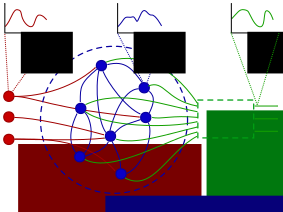
\includegraphics[width=0.6\textwidth]{figures/reservoir}
  \caption{High-level view of a reservoir computer. Each node may have
    three kinds of connections: connections to other nodes in the
    network ($W_r$, blue), connections to the overall input
    ($W_\text{in}$, red), or connections to the output
    ($W_\text{out}$, green). Note that the internal connections may
    contain cycles.  When the RC is used to perform forecasting,
    the output on the right side is connected to the input on the left
    side, allowing the RC to run autonomously with no external
    input.}%
  \label{fig:reservoir}
\end{figure}
% echo state network in particular
% discrete time -- is continuous through euler
% nonlinearity on node or output
% how do you construct the matrices?
% summarize metaparameters (table)

\section{Properties of Good Reservoirs}\label{sec:reservoir-properties}
% summarize known results
% gen sync / fading memory

\section{Evaluating Reserviors}
% NRMSE, inference and forecast
% problems with NRMSE on forecast
% one solution: many trials, and then combine
% other solution: look at attractor and/or return maps
% problem: this is qualitative. how to make quantitative? future research

\section{Summary}
% conclusion: RCs are simple, fast to train, work well. Metaparameters are a
% problem. We will explore that in next chapter!
